\section{Результаты моделирования и экспериментальные исследования}

Верификация синтезированного RTL-тракта и программного окружения проводилась на реальной выборке оцифрованного радиосигнала промежуточной частоты спутниковой радионавигационной системы GPS L1 C/A, зафиксированной в файле \texttt{gps\_if\_signal.bin}[cite: 3].

В процессе работы аппаратного конвейера производился сквозной контроль промежуточных спектральных выборок, выведенных на верхний уровень через диагностические порты \texttt{fft\_out\_re/im} и \texttt{mix\_out\_re/im}[cite: 2]. На рис.~\ref{fig:spectra} представлено сопоставление спектра радиосигнала до и после согласованной фильтрации на частотном срезе $f_d = 0$~Гц[cite: 3].

\begin{figure}[htbp]
    \centering
    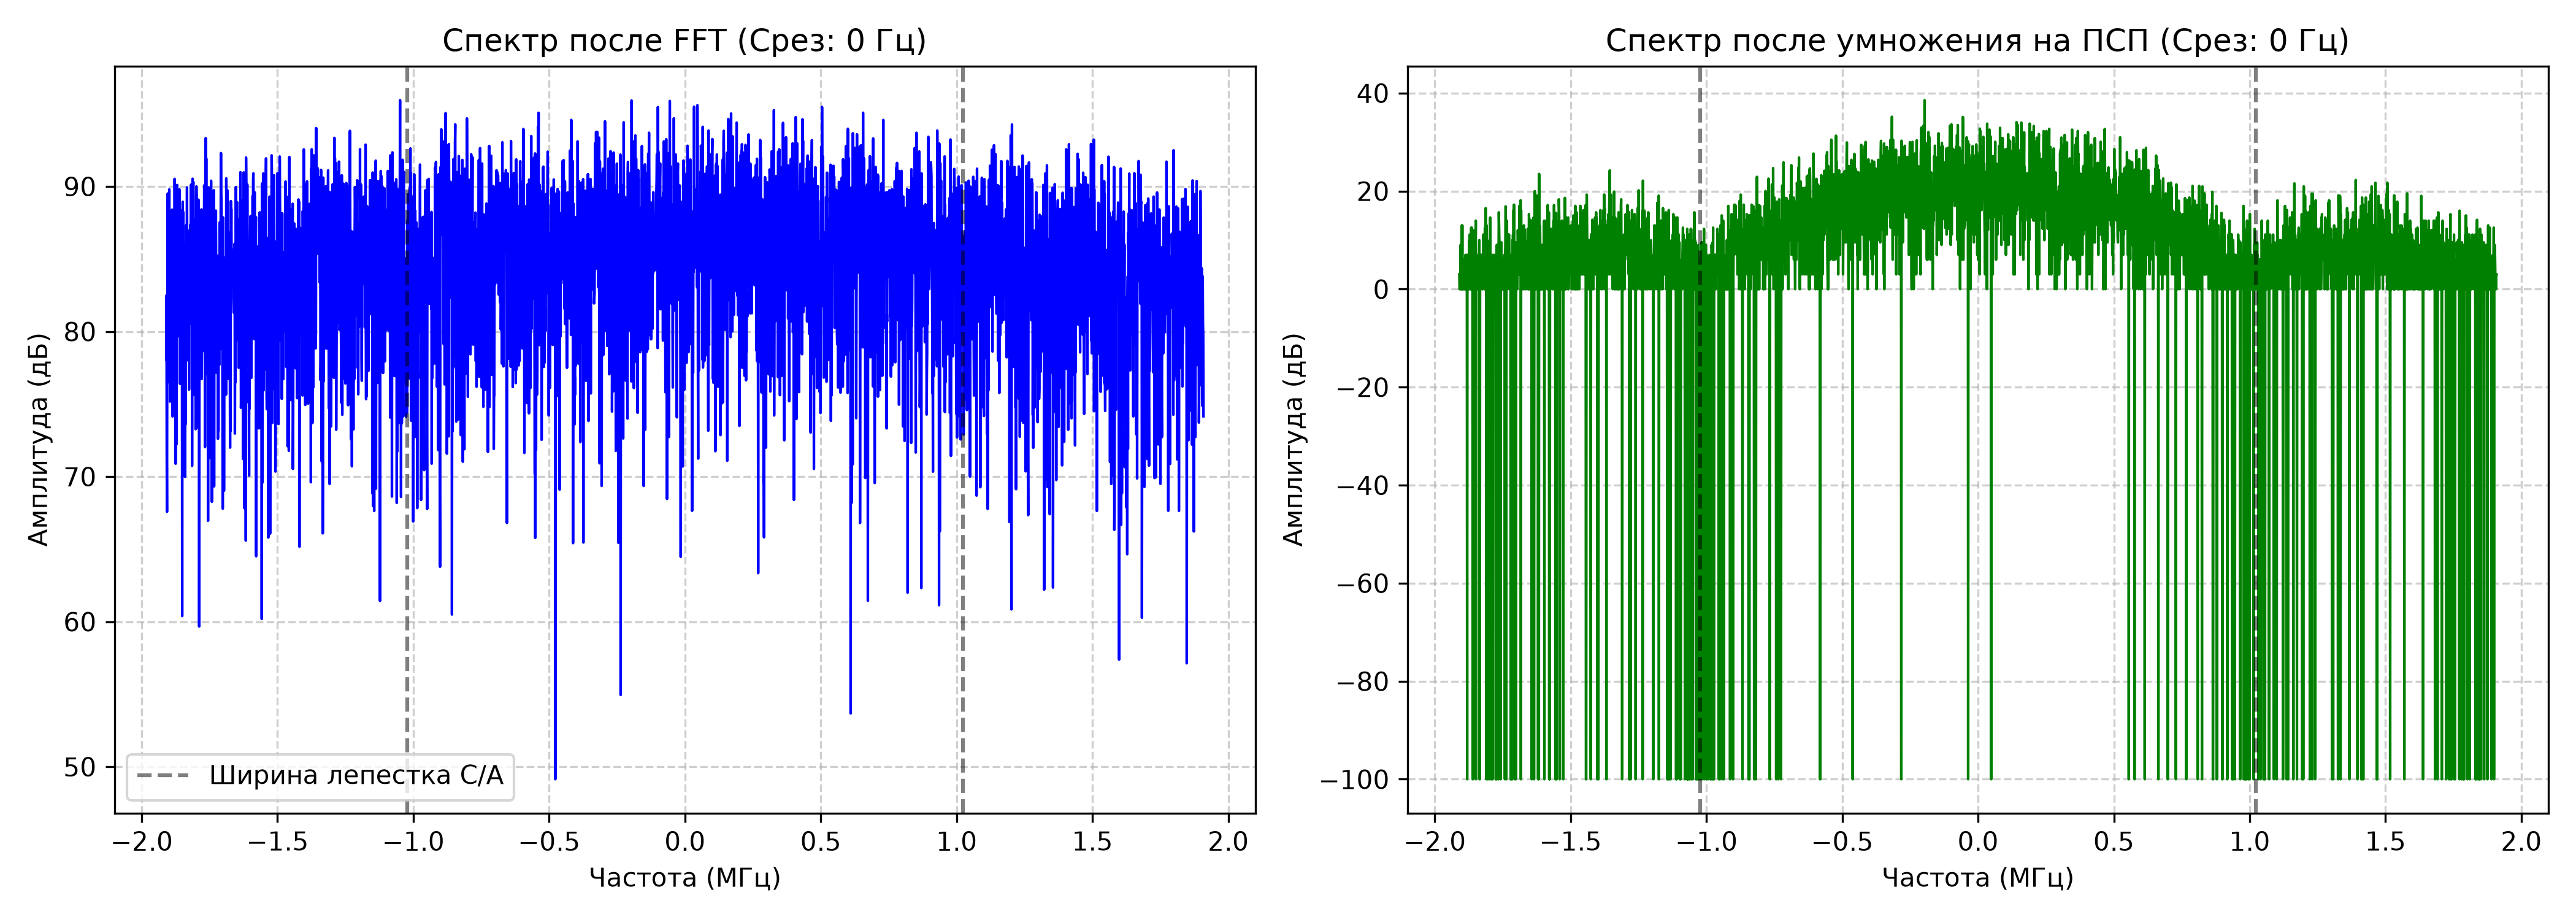
\includegraphics[width=\linewidth]{fig/fig1_spectra.png}
    \caption{Спектральная плотность мощности сигнала на промежуточных каскадах: на выходе прямого БПФ (слева) и после перемножения со спектром опорной ПСП (справа)}
    \label{fig:spectra}
\end{figure}

Спектр на выходе прямого БПФ демонстрирует характерную для подпороговых навигационных сигналов шумовую структуру без выраженных спектральных компонент, что обусловлено отрицательным отношением сигнал/шум до накопления ($-20\dots -30$~дБ). После перемножения комплексного спектра смеси на опорную псевдослучайную последовательность кода Голда в блоке \texttt{spectrum\_multiplier} четко проявляется энергетический главный лепесток шириной 2{,}046~МГц ($\pm 1{,}023$~МГц), соответствующий теоретическому распределению мощности дальномерного кода C/A[cite: 2].

Результаты полного двумерного сканирования пространства поиска по 21 частотному бину в диапазоне от $-5$ до $+5$~кГц с шагом 500~Гц представлены на рис.~\ref{fig:pcps_map}[cite: 3].

\begin{figure}[htbp]
    \centering
    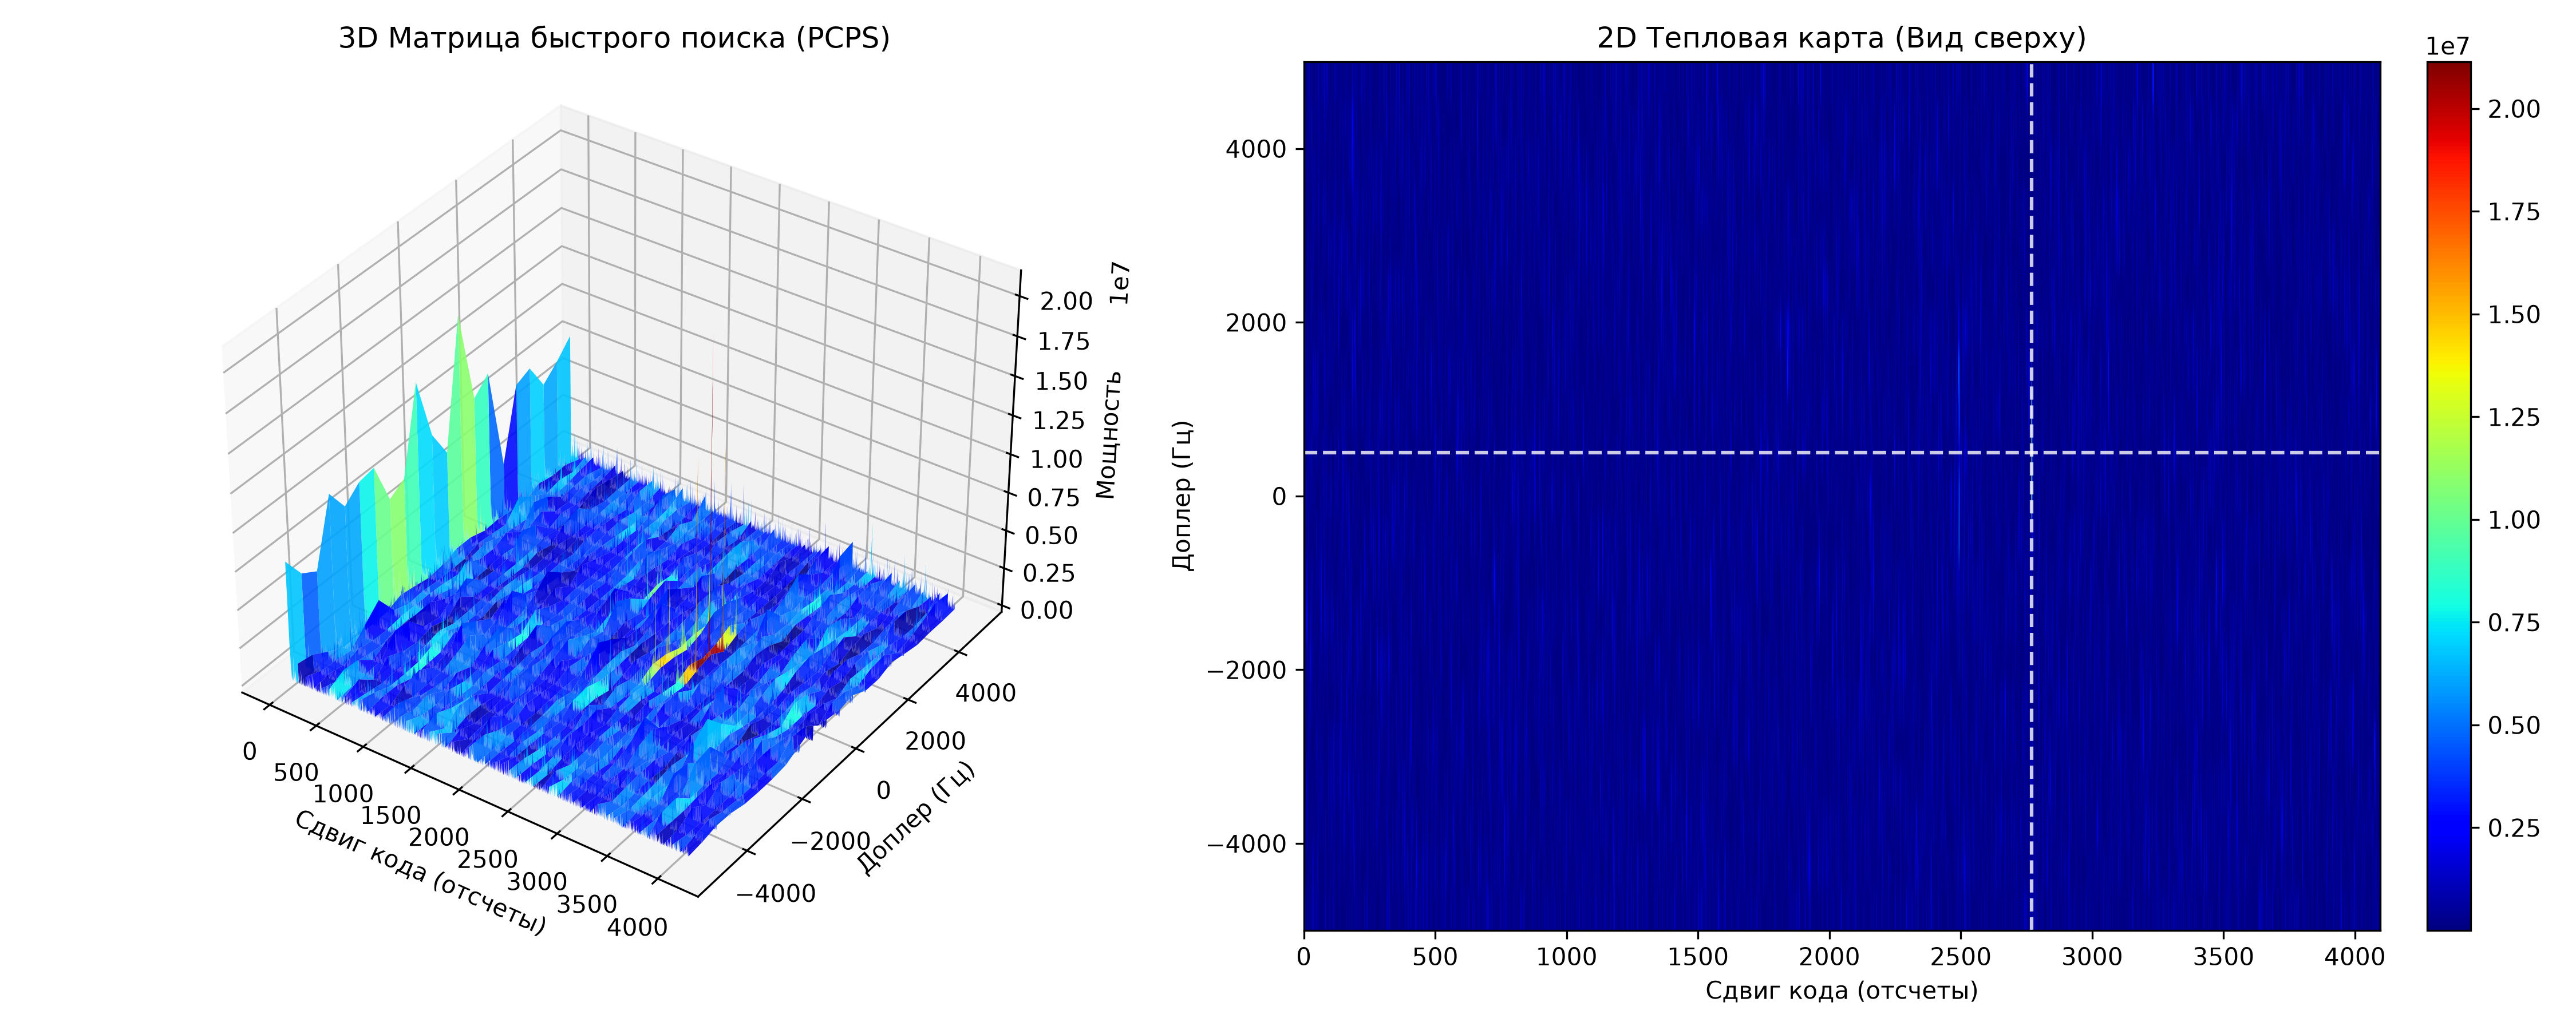
\includegraphics[width=\linewidth]{fig/fig3_acquisition_3d_2d.png}
    \caption{Двумерная функция неопределенности, полученная на выходе детектора мощности \texttt{power\_detector}: 3D-профиль (слева) и проекция на плоскость «задержка -- Доплер» (справа)}
    \label{fig:pcps_map}
\end{figure}

На сформированной тепловой карте однозначно идентифицируется выраженная сингулярность, свидетельствующая о наличии сигнала целевого космического аппарата. Выходной массив мощности квадратичного детектора $I^2 + Q^2$ демонстрирует подавление боковых лепестков взаимной корреляции и шума до уровней, не превышающих $0{,}3\cdot 10^7$, в то время как полезный отклик формирует выраженный экстремум[cite: 2].

\begin{figure}[htbp]
    \centering
    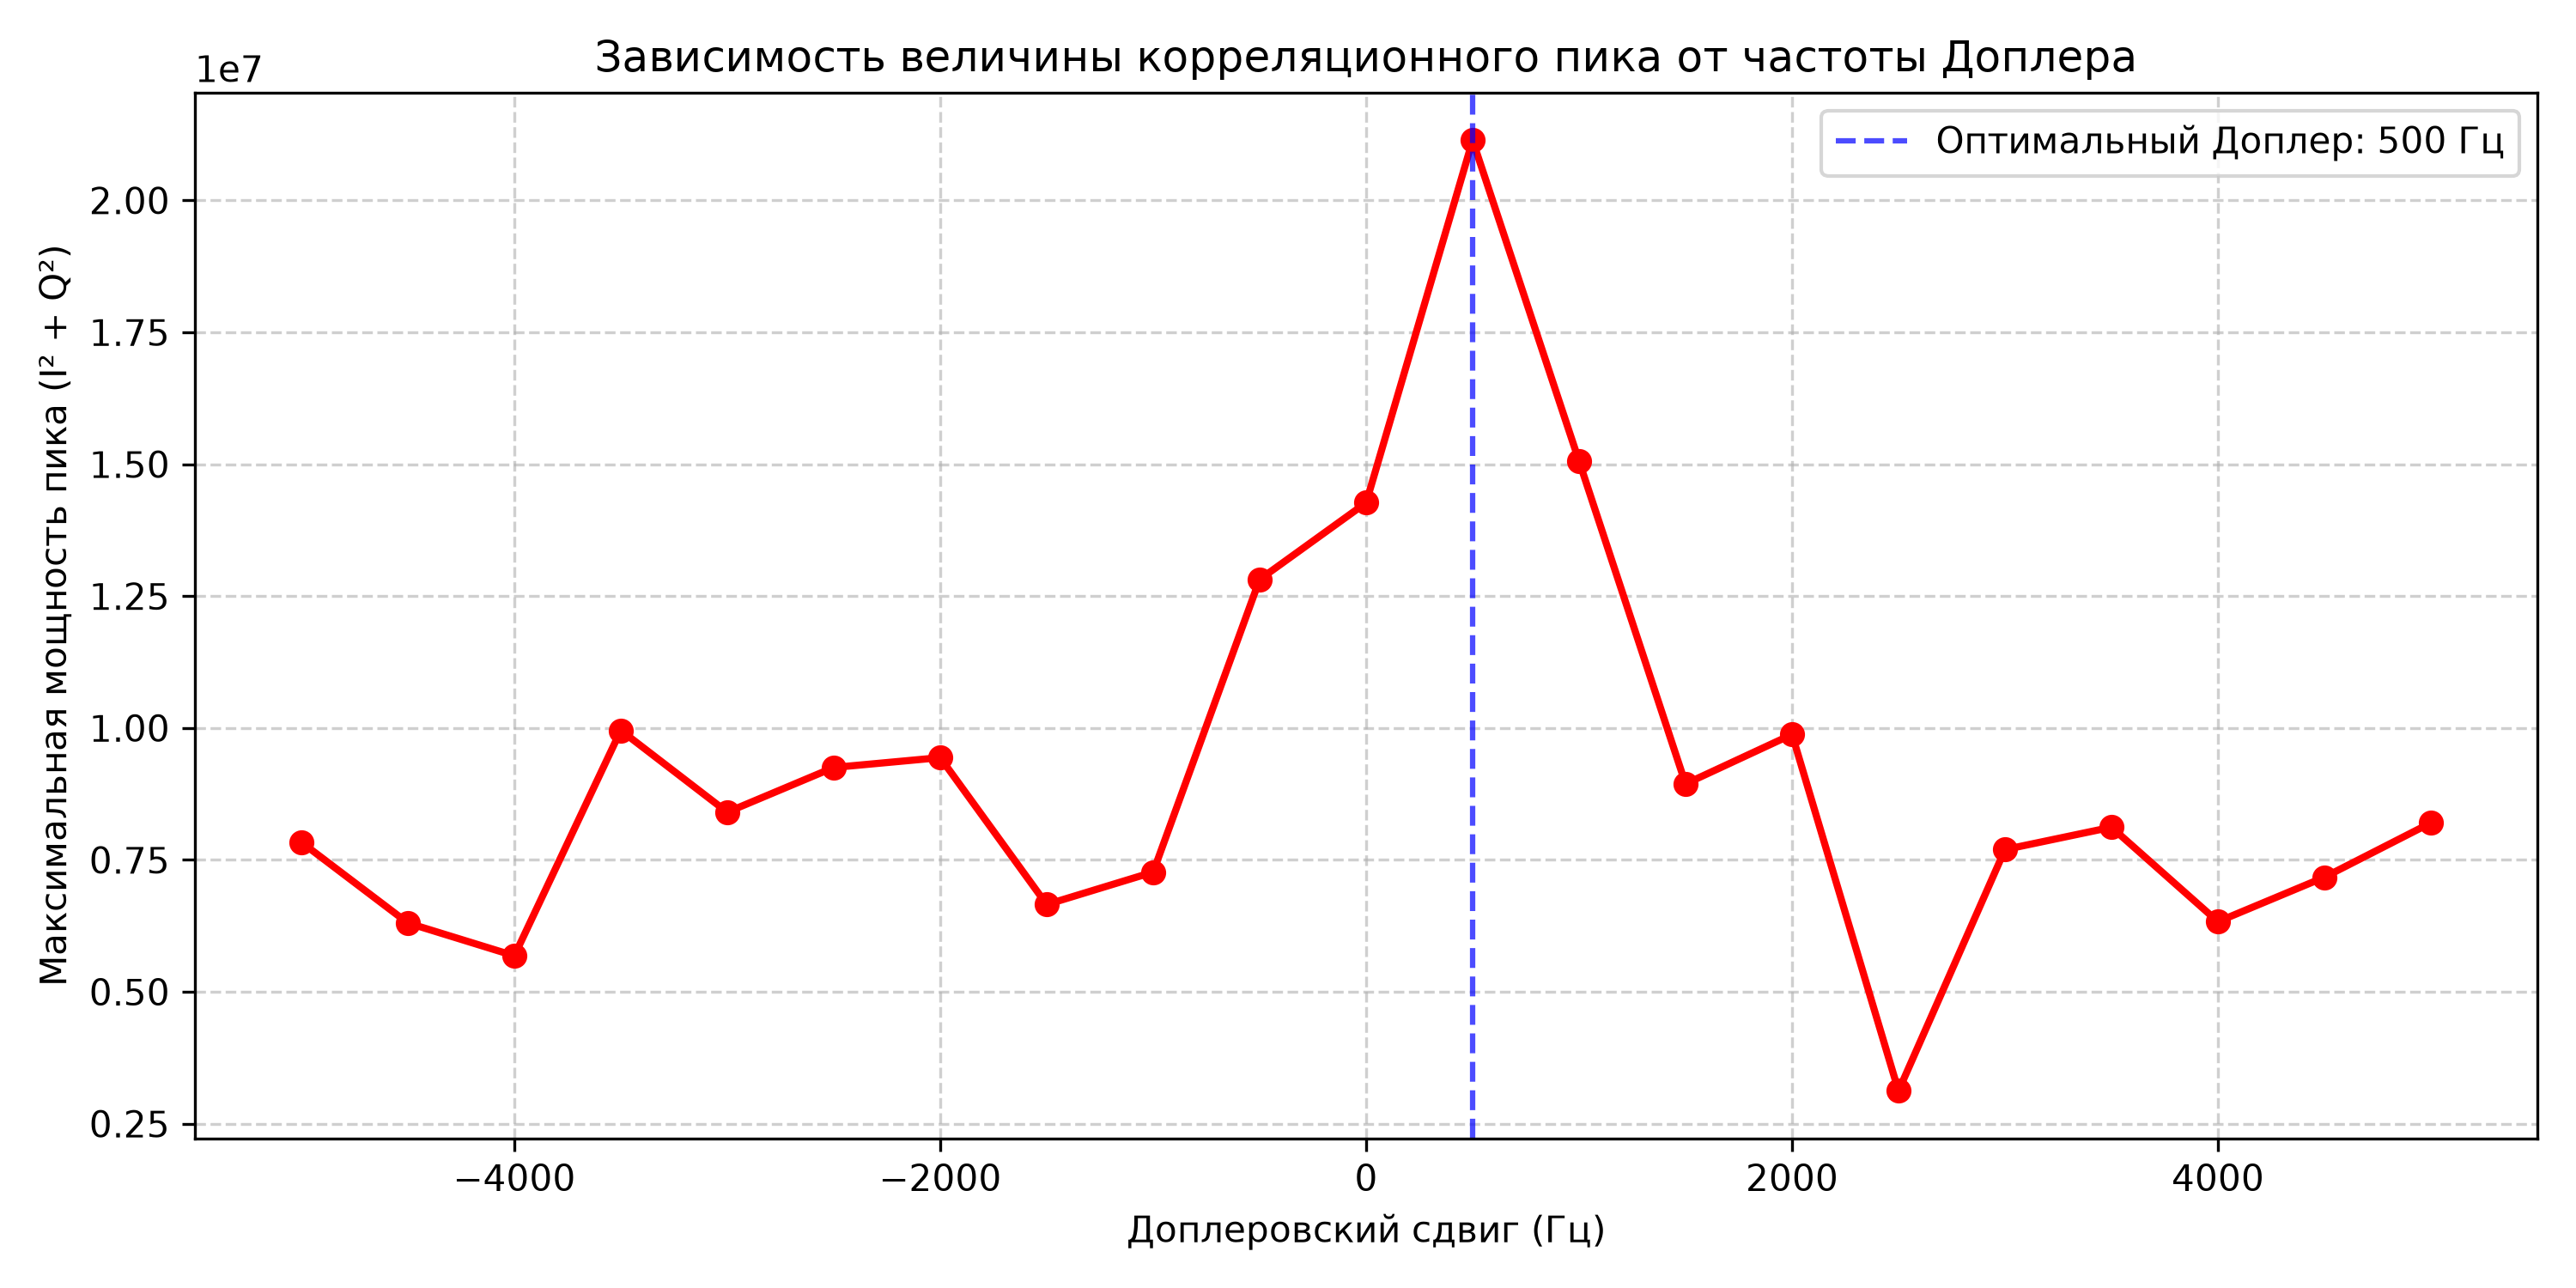
\includegraphics[width=\linewidth]{fig/fig4_peak_vs_doppler.png}
    \caption{Зависимость амплитуды корреляционного максимума от сдвига доплеровской частоты}
    \label{fig:doppler_curve}
\end{figure}

Анализ одномерного частотного среза (рис.~\ref{fig:doppler_curve}) показывает, что максимум энергии регистрируется на частоте Доплера $f_d = +500$~Гц, где величина отклика достигает $2{,}11\cdot 10^7$[cite: 3]. При расстройке на один частотный шаг ($\pm 500$~Гц) наблюдается спад мощности более чем на 30\%, что соответствует передаточной характеристике алгоритма PCPS при длительности когерентного накопления в один период кода Голда ($T_{\text{coh}} = 1$~мс).

\begin{figure}[htbp]
    \centering
    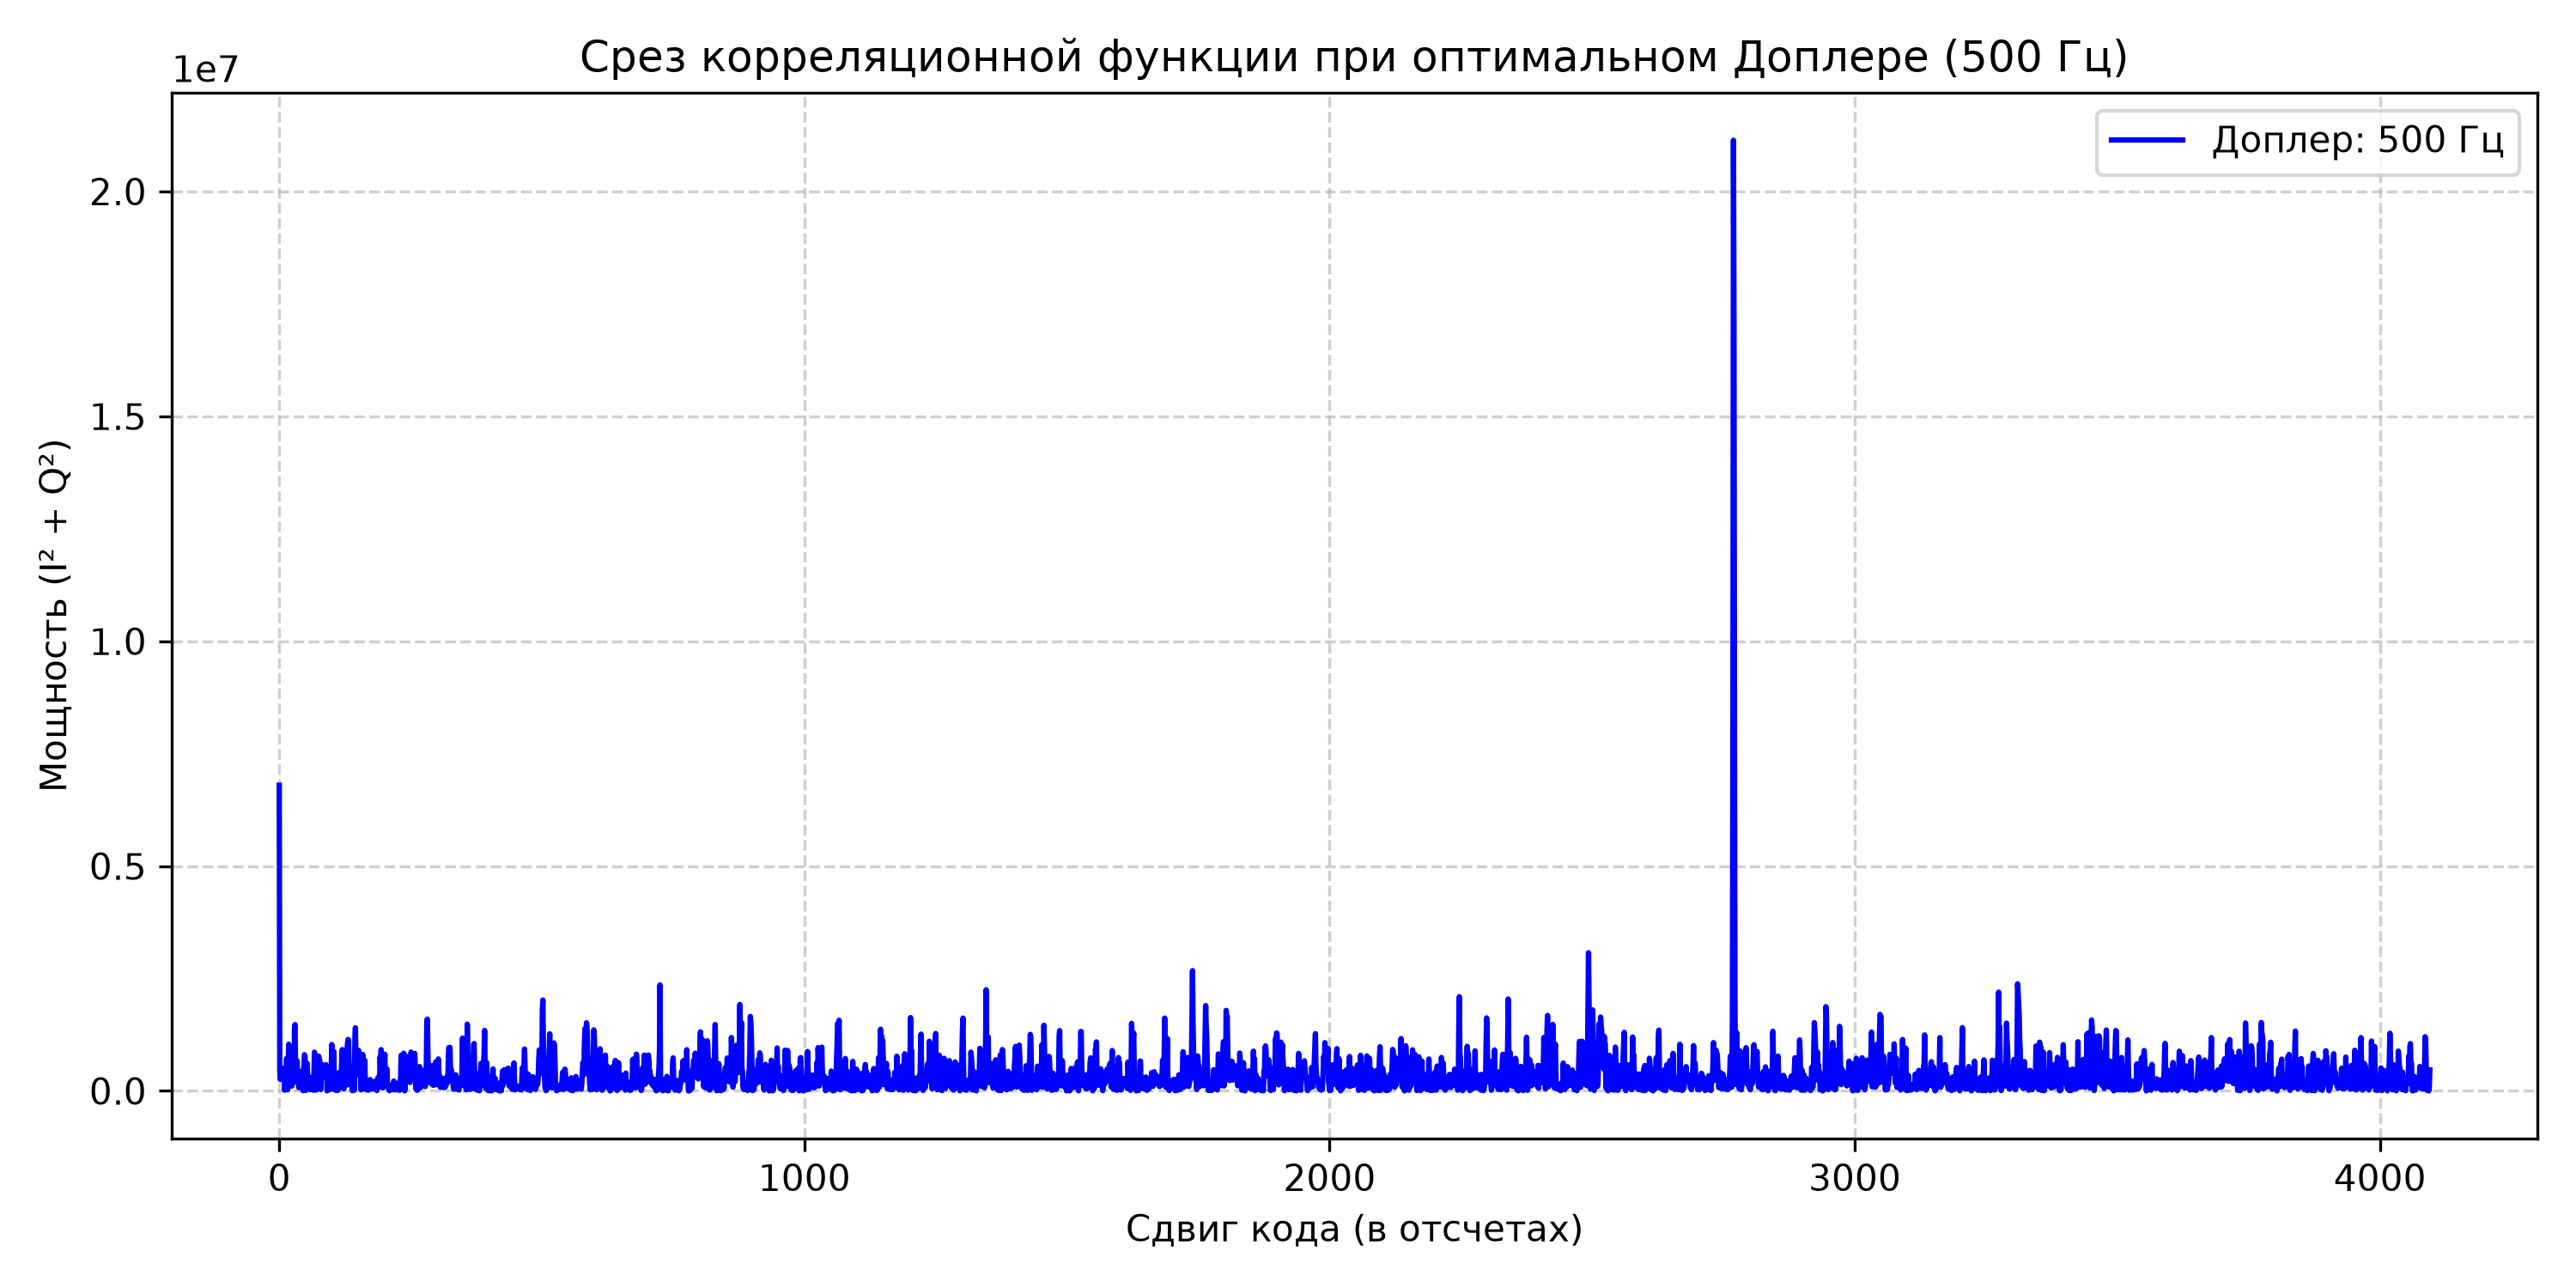
\includegraphics[width=\linewidth]{fig/fig2_doppler_slice.png}
    \caption{Срез корреляционной функции по кодовой задержке в оптимальном частотном канале ($f_d = +500$~Гц)}
    \label{fig:corr_slice}
\end{figure}

На рис.~\ref{fig:corr_slice} приведен временной срез корреляционной функции для оптимального доплеровского бина[cite: 3]. Корреляционный пик зафиксирован на ячейке задержки $\tau = 2768$ отсчетов. Применение программного CFAR-детектора по критерию Неймана--Пирсона с заданной вероятностью ложной тревоги $P_{\text{fa}} = 10^{-5}$ сформировало адаптивный порог обнаружения $V_{\text{th}}$, который был уверенно преодолен экстремумом с расчетным отношением сигнал/шум порядка $18{,}4$~дБ, подтверждая успешный захват сигнала навигационного спутника[cite: 3].
